%% HEADER
%%%%%%%%%%%%%%%%%%%%%%%%%%%%%%%%%%%%%%%%%%%%%%%%%%%%%%%%%%%%%
\newcommand{\hyperrefpdfauthor}{}
\newcommand{\hyperrefpdftitle}{}
\newcommand{\hyperrefpdfsubject}{}
\newcommand{\hyperrefpdfkeywords}{}
\newcommand{\hyperrefpdfborder}{0}
\documentclass{styles/wissdoc-kw-eng}


\usepackage[printonlyused]{acronym}
\renewcommand{\bflabel}[1]{\normalfont{\normalsize{#1}}\hfill} % keine serifenlose schrift für acronym
%\usepackage{acronym}
\usepackage{subfigure}

\usepackage{float}
\floatstyle{ruled}
\newfloat{listing}{htbp}{lop}[chapter]
\floatname{listing}{Listing}

\usepackage[hang,center,nooneline]{caption}
\captionsetup[figure]{font={small,sf}}
\captionsetup[table]{font={small,sf}}
\captionsetup[listing]{font={small,sf}}
\usepackage{etoolbox}


%% Normales LaTeX oder pdfLaTeX? %%%%%%%%%%%%%%%%%%%%%%%%%%%%
%% ==> Das neue if-Kommando "\ifpdf" wird an einigen wenigen
%% ==> Stellen benötigt, um die Kompatibilität zwischen
%% ==> LaTeX und pdfLaTeX herzustellen.
%\newif\ifpdf
%\ifx\pdfoutput\undefined
%    \pdffalse              %%normales LaTeX wird ausgeführt
%\else
%    \pdfoutput=1
%    \pdftrue               %%pdfLaTeX wird ausgeführt
%\fi


%% Fonts für pdfLaTeX %%%%%%%%%%%%%%%%%%%%%%%%%%%%%%%%%%%%%%%
%% ==> Nur notwendig, falls keine cm-super-Fonts installiert
\ifpdf
	\usepackage{ae}       %%Benutzen Sie nur eines dieser Pakete:
	%\usepackage{zefonts}  %%je nachdem, welches Sie besitzen.
\else
	%%Normales LaTeX - keine speziellen Fontpackages notwendig
\fi


%% Deutsche Anpassungen %%%%%%%%%%%%%%%%%%%%%%%%%%%%%%%%%%%%%
%\usepackage[T1]{fontenc}
%\usepackage[utf8]{inputenc}

%% zur Zitaten des Quelltextes%%%%%%%%%%%%%%%%%%%%%%%%%%%%%%%
% "final" forces printing of all listings, even if the global "draft" is set
\usepackage[final]{listings}
\lstset{
    basicstyle=\footnotesize\ttfamily,
    tabsize=4,
    numberstyle=\tiny\color{gray},
    numbersep=5pt,
    numbers=left,
    captionpos=b,
    abovecaptionskip=0pt,
    belowcaptionskip=0pt,
    aboveskip=10pt,
    belowskip=0pt,
    floatplacement=tbp,
    frame=topline,
    framerule=.1pt,
    framesep = 3pt,
    }
\renewcommand\lstlistingname{\textbf{Listing}}
% This is only kept for backwards compatibility. You should never have to use it. Use the listing-environment instead.
%\DeclareCaptionFormat*{lstruled}{{\bfseries#1\small\space\normalfont#3\hrule height.1pt depth0pt}\par}
%\captionsetup[lstlisting]{format=lstruled,singlelinecheck=false}

%% mehrere Abbildungen in eine %%%%%%%%%%%%%%%%%%%%%%%%%%%%%%
\usepackage{subfigure}

%% Packages für Formeln %%%%%%%%%%%%%%%%%%%%%%%%%%%%%%%%%%%%%
\usepackage{amsmath}
\usepackage{amsthm}
\usepackage{amsfonts}

%% Zeilenabstand %%%%%%%%%%%%%%%%%%%%%%%%%%%%%%%%%%%%%%%%%%%%
\usepackage{setspace}
%\singlespacing        %% 1-zeilig (Standard)
%\onehalfspacing       %% 1,5-zeilig
%\doublespacing        %% 2-zeilig


%% Andere Packages %%%%%%%%%%%%%%%%%%%%%%%%%%%%%%%%%%%%%%%%%%
%\usepackage{a4wide} %%Kleinere Seitenränder = mehr Text pro Zeile.
\usepackage{fancyhdr} %%Fancy Kopf- und Fußzeilen
%\usepackage{longtable} %%Für Tabellen, die eine Seite überschreiten
\usepackage{lscape}
\usepackage{rotating} 
%\usepackage[htt]{hyphenat} %Trennung von Typewriter-Schriften
%\usepackage{listings}
\usepackage{pstricks-add}


% Tabellen mit Center und left
\usepackage{tabularx,colortbl} % colored table background
\newcolumntype{C}[1]{>{\centering\arraybackslash}p{#1}}
\newcolumntype{R}[1]{>{\raggedleft\arraybackslash}p{#1}}
% Table spacings
\newcommand\T{\rule{0pt}{2.5ex}\rule[-1.0ex]{0pt}{0pt}}
\newcommand\B{\rule[-1.0ex]{0pt}{0pt}}

\definecolor{slightgray}{gray}{.90} 


%% Definitionen %%%%%%%%%%%%%%%%%%%%%%%%%%%%


%% zur Benutzung bei ergänzenden Daten%%%%%%%%%%%%%%%%%%%%%%%%
%\usepackage{endnotes}
%\renewcommand{\notesname}{Konfigurationsdaten der Messreihen}
%\renewcommand{\theendnote}{\Alph{endnote}}
%\renewcommand{\enotesize}{\normalsize}

%\hyphenation{Sensor-netz-werk
%}

%%%%%%%%%%%%%%%%%%%%%%%%%%%%%%%%%%%%%%%%%%%%%%%%%%%%%%%%%%%%%
%% DOKUMENT
%%%%%%%%%%%%%%%%%%%%%%%%%%%%%%%%%%%%%%%%%%%%%%%%%%%%%%%%%%%%%
\begin{document}

%% Dateiendungen für Grafiken %%%%%%%%%%%%%%%%%%%%%%%%%%%%%%%
%% ==> Sie können hiermit die Dateiendung einer Grafik weglassen.
%% ==> Aus "\includegraphics{titel.eps}" wird "\includegraphics{titel}".
%% ==> Wenn Sie nunmehr 2 inhaltsgleiche Grafiken "titel.eps" und
%% ==> "titel.pdf" erstellen, wird jeweils nur die Grafik eingebunden,
%% ==> die von ihrem Compiler verarbeitet werden kann.
%% ==> pdfLaTeX benutzt "titel.pdf". LaTeX benutzt "titel.eps".
%\ifpdf
%    \DeclareGraphicsExtensions{.pdf,.jpg,.png}
%\else
%    \DeclareGraphicsExtensions{.eps}
%\fi

\pagestyle{empty} %%Keine Kopf-/Fusszeilen auf den ersten Seiten.

\ifnotdraft{
%% Deckblatt %%%%%%%%%%%%%%%%%%%%%%%%%%%%%%%%%%%%%%%%%%%%%%%%
\frontmatter
\titlehead{
	\centering
	
\includegraphics[height=20mm,keepaspectratio]{logos/comsys-text}
	\hfill
	
\includegraphics[height=20mm,keepaspectratio]{logos/rwth}
} % end titlehead

\begin{titlepage}

\let\footnotesize\small \let\footnoterule\relax

\hbox{}
\vfill

\centering

\begin{doublespace}
{ \huge\textbf{\textsf{Robust Wireless Link and Channel Assignment Algorithm
Minimizing Interference Utilizing Multi-Radio Access Points 
}}}
%{ \huge\textbf{\textsf{Your Awesome Thesis Title \\ \vspace{-0.4em}
%(Which May Also Be Long \\ \vspace{0.4em}
%And Stretch multiple Lines) Here}}}
\end{doublespace}
\vskip 2cm

{\large Bachelor Thesis\\[5pt]}
{\large \textbf{Konstantin Manna}}
\vskip 1cm

\textbf{RWTH Aachen University, Germany\\[5pt]
        Chair of Communication and Distributed Systems}
\vskip 2cm

\large

Advisors:
\vskip 2mm

\begin{tabular}{R{7cm}p{7cm}}
Dipl.-Inform. & Christoph Wollgarten\\
Dipl.-Inform. & J\'o \'Agila Bitsch Link\\
Prof.~Dr.-Ing. & Klaus Wehrle\\
Prof.~Dr. & Bernhard Rumpe
\end{tabular}
\vskip 1cm

\begin{tabular}{R{6cm}p{6cm}}
Registration date:  & 2014-05-20 \\
Submission date:    & 2014-09-22 \\
\end{tabular}

\vfill

\end{titlepage}


\cleardoublepage
\thispagestyle{empty}
\vspace*{36\baselineskip}
\hbox to \textwidth{\hrulefill}

I hereby affirm that I composed this work independently and used no other than the specified sources and tools and that I marked all quotes as such.

Hiermit versichere ich, dass ich die Arbeit selbstständig verfasst und keine anderen als die angegebenen Quellen und Hilfsmittel benutzt sowie Zitate kenntlich gemacht habe.

Aachen, den 2. März 2011

\cleardoublepage
\cleardoublepage

\begin{center}
\paragraph{Kurzfassung}
\hrulefill
\end{center}
What is it? \newline
What does it do?\newline
How does it work generally?\newline
Where is it used? \newline
Short Results\newline
\vspace {2cm}
\begin{center}
\paragraph{Abstract}
\hrulefill
\end{center}
\cleardoublepage
\cleardoublepage

\chapter*{Acknowledgments}

I would like to thank Christoph Wollgarten at LANCOM Systems for enabling and supervising this thesis, who despite his huge workload always had a few minutes to spare
to help me with my problems and create the AutoWDSstatus tool, which was much appreciated.
I also want to thank J\'o \'Agila Bitsch for supervising this thesis at COMSYS and his great feedback on this work during several meetings.
Furthermore i want to express my gratitude to Paul Smith who had some tipps and templates for writing this thesis.
Last but not least I thank Prof. Wehrle and Prof. Rumpe for giving me the chance to to write this thesis.
\cleardoublepage

% Titelseite hatte noch normale Tabellen. Von hier ab sollen alle
% Tabellen laut style-Vorgaben sans serif sein.
\AtBeginEnvironment{tabular}{\sffamily}
\AtBeginEnvironment{tabularx}{\sffamily}

%% Inhaltsverzeichnis %%%%%%%%%%%%%%%%%%%%%%%%%%%%%%%%%%%%%%%
\tableofcontents %Inhaltsverzeichnis
\cleardoublepage %Das erste Kapitel soll auf einer ungeraden Seite beginnen.
} % end ifnotdraft

\pagestyle{fancy} %%Ab hier die Kopf-/Fusszeilen: headings / fancy / ...

%%%%%%%%%%%%%%%%%%%%%%%%%%%%%%%%%%%%%%%%%%%%%%%%%%%%%%%%%%%%%
% einzelne Kapitel
%%%%%%%%%%%%%%%%%%%%%%%%%%%%%%%%%%%%%%%%%%%%%%%%%%%%%%%%%%%%%
%\include{commands}

\mainmatter
\chapter{Introduction}



General intro that your non-cs friends also understand
2 to 3 pages

general context of your work
what is it good for
societal relevance.












This is the introduction. Lorem ipsum dolor sit amet, consectetur adipiscing elit. Vestibulum posuere vehicula lorem id commodo. Nam tempor felis quis orci tincidunt suscipit. Morbi dictum purus et nisl porttitor fringilla. Quisque feugiat, tellus quis semper placerat, lectus eros rutrum ipsum, eu elementum nibh nulla eu purus. Vestibulum ultrices varius orci, vitae porta elit laoreet at. Phasellus luctus aliquam molestie. Praesent varius blandit felis eu pellentesque. Aliquam erat volutpat. Morbi at est nibh.

Sed a mi tellus, id pellentesque neque. Integer vel volutpat diam. Sed nec lorem eu arcu lobortis porta. Sed quam nunc, luctus quis facilisis nec, aliquet nec mauris. Mauris non velit nisi, sed convallis risus. Sed quis lectus ligula. Morbi in nibh elit. Aenean a purus justo. Suspendisse pretium semper faucibus. Proin dictum, justo quis sagittis cursus, erat massa sollicitudin magna, in tempus quam lacus non turpis.

Cum sociis natoque penatibus et magnis dis parturient montes, nascetur ridiculus mus. Etiam congue magna at est pellentesque nec hendrerit arcu aliquet. Vivamus sem lectus, vehicula elementum accumsan iaculis, condimentum a mi. Proin sit amet justo eleifend massa eleifend lacinia. Mauris nibh nisl, vehicula vel tincidunt ac, varius et odio. Aliquam feugiat nulla ac felis interdum sodales. Etiam mollis arcu et mi scelerisque quis viverra est vestibulum. Mauris at massa libero, sit amet tincidunt elit. Mauris tempor lorem ut purus hendrerit non viverra nisi vehicula.

Vivamus ligula dui, semper sed consequat non, tempor ut diam. Morbi metus nisl, adipiscing feugiat malesuada viverra, blandit id nunc. Aliquam sed ante id velit ultricies condimentum. Aenean lacinia elementum lacus sit amet luctus. Vestibulum consequat nibh et tortor laoreet sit amet vehicula orci venenatis. Suspendisse enim velit, hendrerit quis vestibulum sit amet, tincidunt sit amet odio. Sed gravida tellus in nunc egestas porta. Morbi suscipit, dui vel elementum volutpat, lectus nulla elementum lacus, vitae dictum erat turpis ut ligula. Donec sit amet dolor ut urna vestibulum consequat nec et purus. In adipiscing lacus vel tellus fermentum quis cursus sapien egestas. Curabitur id ipsum erat. In lacinia adipiscing sapien at varius.

In consequat laoreet blandit. Ut ac ipsum at velit malesuada tincidunt ornare at sapien. Aenean at dui dolor. Pellentesque sit amet fermentum lorem. Nullam pulvinar diam eget diam hendrerit condimentum. Duis fermentum vulputate ante, a egestas mauris vehicula at. Quisque convallis vestibulum fermentum. Aenean molestie dictum libero, a tincidunt lectus vestibulum in. Vivamus consequat purus pellentesque urna elementum consequat. Cras nec tortor felis, ac cursus risus. Morbi gravida ligula nec orci aliquam aliquam. Morbi et ligula diam, vel venenatis eros. Duis rhoncus ultricies mollis. Nullam ut est lacinia est auctor consectetur faucibus nec tellus. Phasellus id tincidunt risus. Nulla volutpat quam vel diam vehicula in egestas ligula laoreet. 

\begin{listing}[t]
\begin{lstlisting}
#include <stdio.h>

int main(void)
{
	printf("Hello, World\n");

	return 0;
}
\end{lstlisting}
\caption{A simple code example.}
\label{lst:example}
\end{listing}

Lorem ipsum dolor sit amet, consectetur adipiscing elit. Vestibulum posuere vehicula lorem id commodo. Nam tempor felis quis orci tincidunt suscipit. Morbi dictum purus et nisl porttitor fringilla. Quisque feugiat, tellus quis semper placerat, lectus eros rutrum ipsum, eu elementum nibh nulla eu purus. Vestibulum ultrices varius orci, vitae porta elit laoreet at. Phasellus luctus aliquam molestie. Praesent varius blandit felis eu pellentesque. Aliquam erat volutpat. Morbi at est nibh.

Sed a mi tellus, id pellentesque neque. Integer vel volutpat diam. Sed nec lorem eu arcu lobortis porta. Sed quam nunc, luctus quis facilisis nec, aliquet nec mauris. Mauris non velit nisi, sed convallis risus. Sed quis lectus ligula. Morbi in nibh elit. Aenean a purus justo. Suspendisse pretium semper faucibus. Proin dictum, justo quis sagittis cursus, erat massa sollicitudin magna, in tempus quam lacus non turpis.

Cum sociis natoque penatibus et magnis dis parturient montes, nascetur ridiculus mus. Etiam congue magna at est pellentesque nec hendrerit arcu aliquet. Vivamus sem lectus, vehicula elementum accumsan iaculis, condimentum a mi. Proin sit amet justo eleifend massa eleifend lacinia. Mauris nibh nisl, vehicula vel tincidunt ac, varius et odio. Aliquam feugiat nulla ac felis interdum sodales. Etiam mollis arcu et mi scelerisque quis viverra est vestibulum. Mauris at massa libero, sit amet tincidunt elit. Mauris tempor lorem ut purus hendrerit non viverra nisi vehicula.

Vivamus ligula dui, semper sed consequat non, tempor ut diam. Morbi metus nisl, adipiscing feugiat malesuada viverra, blandit id nunc. Aliquam sed ante id velit ultricies condimentum. Aenean lacinia elementum lacus sit amet luctus. Vestibulum consequat nibh et tortor laoreet sit amet vehicula orci venenatis. Suspendisse enim velit, hendrerit quis vestibulum sit amet, tincidunt sit amet odio. Sed gravida tellus in nunc egestas porta. Morbi suscipit, dui vel elementum volutpat, lectus nulla elementum lacus, vitae dictum erat turpis ut ligula. Donec sit amet dolor ut urna vestibulum consequat nec et purus. In adipiscing lacus vel tellus fermentum quis cursus sapien egestas. Curabitur id ipsum erat. In lacinia adipiscing sapien at varius.

\begin{figure}[t]
\centering
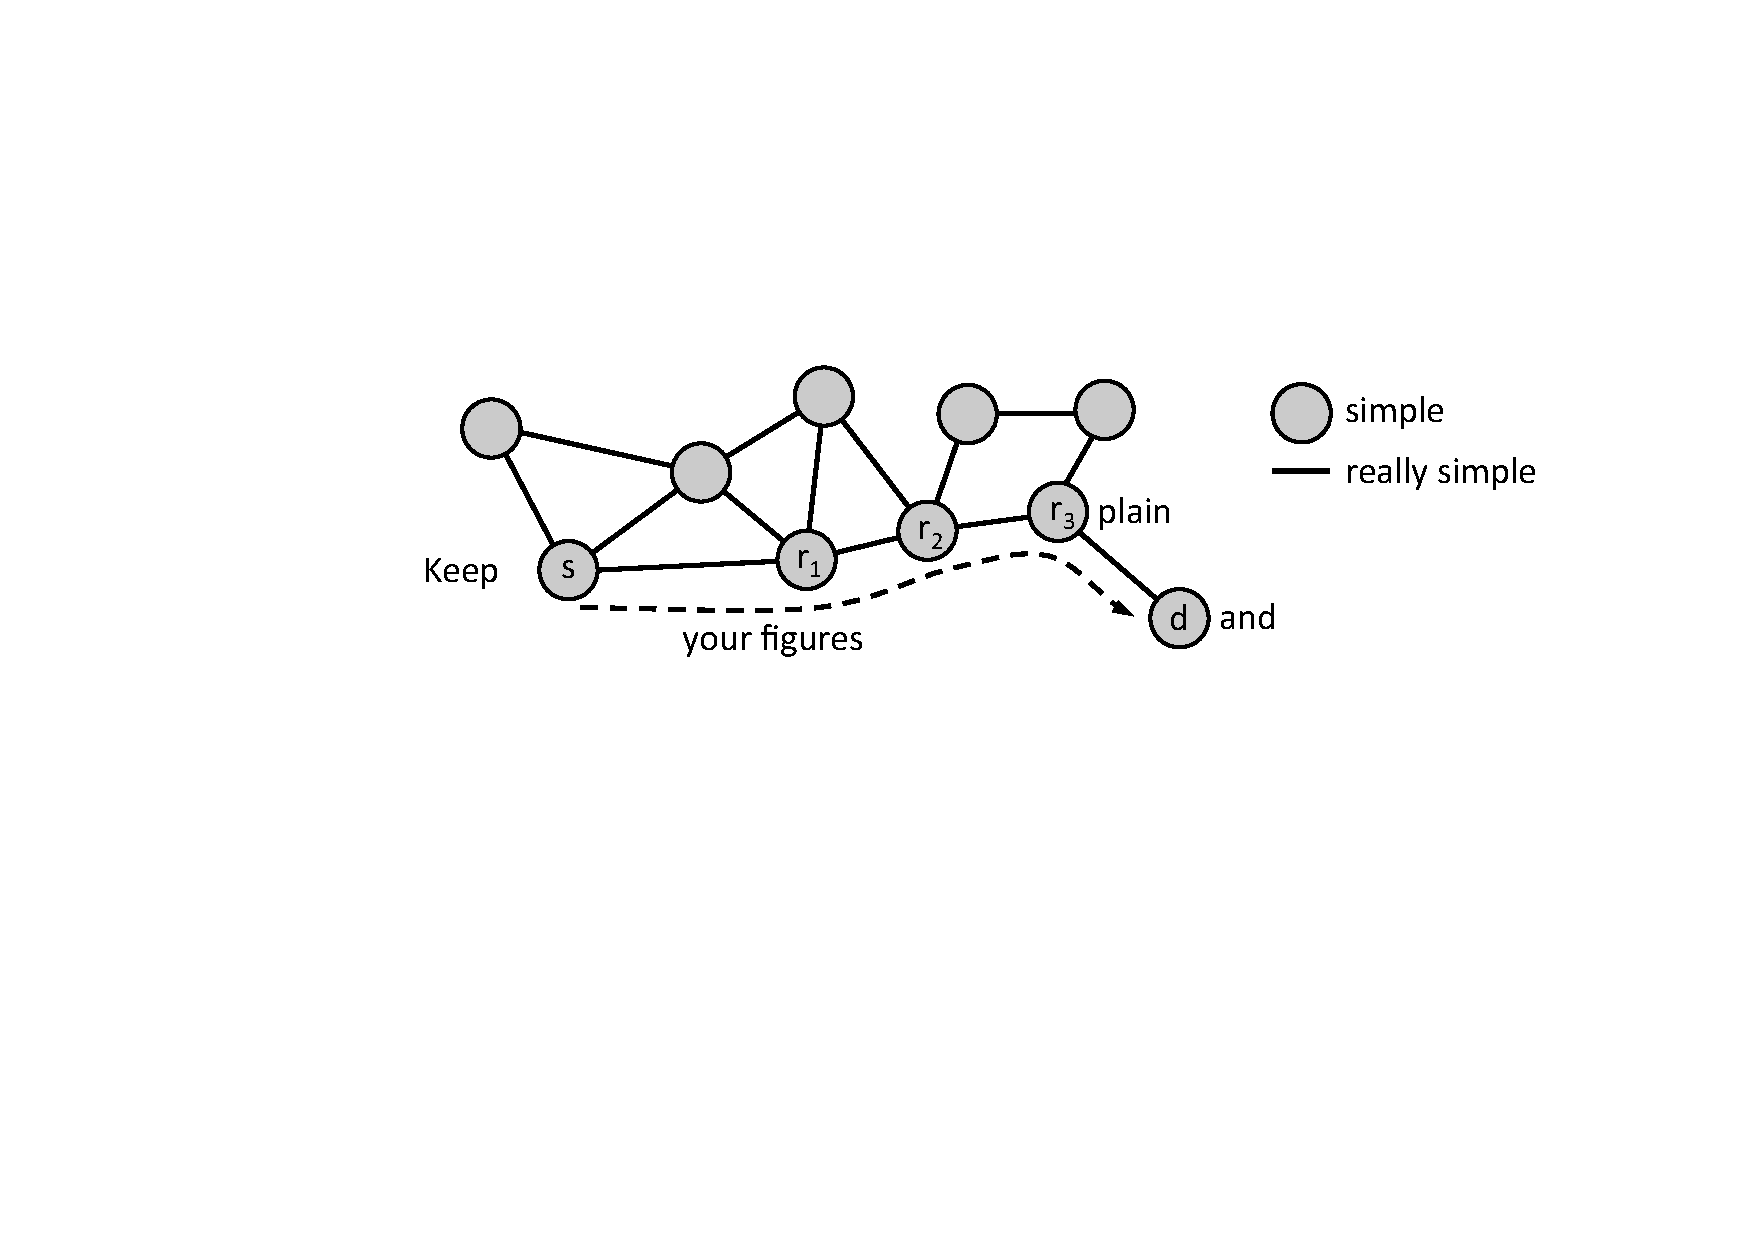
\includegraphics[width=1\columnwidth]{figures/example}
\caption{An example of an awesome image!}
\label{fig:example}
\end{figure} 


Maecenas non tortor lorem, ac cursus nulla. Ut accumsan, felis vitae sollicitudin imperdiet, magna magna semper neque, faucibus feugiat augue neque vel risus. Quisque suscipit pellentesque felis, quis commodo felis mattis et. Maecenas ac augue sed enim posuere facilisis. Nam fringilla faucibus blandit. Morbi ante nisi, sodales in laoreet eu, fermentum sit amet tellus. Integer vel lorem turpis, eu commodo augue. Etiam vel tellus velit, et hendrerit magna. Nulla vitae tellus ut odio pellentesque varius eu eget turpis. In eros neque, rhoncus ac imperdiet eu, luctus eget mi.

Nulla sed lectus pulvinar tellus pretium dignissim pretium in dolor. Sed mollis ornare nisi. Nulla facilisi. Sed porta venenatis ultrices. Sed ut libero nec arcu lobortis suscipit non eget lacus. Donec egestas lacinia ligula, quis tristique eros dapibus eget. Suspendisse iaculis felis id lacus vestibulum malesuada. In vel tincidunt dui. In sed sapien nulla, sit amet venenatis felis. Integer quis leo ipsum, ac sagittis nibh. Curabitur interdum, turpis eu tincidunt ornare, arcu justo aliquet est, ut congue tortor dolor eget leo. Morbi viverra iaculis porttitor. Maecenas eleifend varius tellus, id ultricies sem dapibus id. Fusce lacinia arcu ac odio varius ac ultricies erat mollis. Lorem ipsum dolor sit amet, consectetur adipiscing elit. 

\begin{description}
\item[Ut ac ipsum:]
Ut ac ipsum at velit malesuada tincidunt ornare at sapien. Aenean at dui dolor. Pellentesque sit amet fermentum lorem. Nullam pulvinar diam eget diam hendrerit condimentum. Duis fermentum vulputate ante, a egestas mauris vehicula at. Quisque convallis vestibulum fermentum.

\item[Aenean lacinia elementum:]
Aliquam sed ante id velit ultricies condimentum. Aenean lacinia elementum lacus sit amet luctus. Vestibulum consequat nibh et tortor laoreet sit amet vehicula orci venenatis. Suspendisse enim velit, hendrerit quis vestibulum sit amet, tincidunt sit amet odio.

\item[Phasellus id:]
Nullam ut est lacinia est auctor consectetur faucibus nec tellus. Phasellus id tincidunt risus. Nulla volutpat quam vel diam vehicula in egestas ligula laoreet. 

\end{description}

In consequat laoreet blandit. Ut ac ipsum at velit malesuada tincidunt ornare at sapien. Aenean at dui dolor. Pellentesque sit amet fermentum lorem. Nullam pulvinar diam eget diam hendrerit condimentum. Duis fermentum vulputate ante, a egestas mauris vehicula at. Quisque convallis vestibulum fermentum. Aenean molestie dictum libero, a tincidunt lectus vestibulum in. Vivamus consequat purus pellentesque urna elementum consequat. Cras nec tortor felis, ac cursus risus. Morbi gravida ligula nec orci aliquam aliquam. Morbi et ligula diam, vel venenatis eros. Duis rhoncus ultricies mollis. Nullam ut est lacinia est auctor consectetur faucibus nec tellus. Phasellus id tincidunt risus. Nulla volutpat quam vel diam vehicula in egestas ligula laoreet. 

\begin{table}[b]
\caption{Tables should look like this (save for the last row). If you know LaTeX better than me, feel free to improve the way of producing these tables.}
\begin{tabularx}{\linewidth}{|l|X|X|}
\hline
\rowcolor{slightgray}
\T Tables	&have gray  &headlines\\
\hline
\cellcolor{slightgray}\T and gray &labels \B&, too.\\
\hline
\cellcolor{slightgray}\T T &and B& are used for spacing\B\\
\hline
\cellcolor{slightgray} without T & and B& the cells are too small\B\\
\hline 
\end{tabularx}
\label{tab:example}
\end{table}

Lorem ipsum dolor sit amet, consectetur adipiscing elit. Vestibulum posuere vehicula lorem id commodo. Nam tempor felis quis orci tincidunt suscipit. Morbi dictum purus et nisl porttitor fringilla. Quisque feugiat, tellus quis semper placerat, lectus eros rutrum ipsum, eu elementum nibh nulla eu purus. Vestibulum ultrices varius orci, vitae porta elit laoreet at. Phasellus luctus aliquam molestie. Praesent varius blandit felis eu pellentesque. Aliquam erat volutpat. Morbi at est nibh.

Sed a mi tellus, id pellentesque neque. Integer vel volutpat diam. Sed nec lorem eu arcu lobortis porta. Sed quam nunc, luctus quis facilisis nec, aliquet nec mauris. Mauris non velit nisi, sed convallis risus. Sed quis lectus ligula. Morbi in nibh elit. Aenean a purus justo. Suspendisse pretium semper faucibus. Proin dictum, justo quis sagittis cursus, erat massa sollicitudin magna, in tempus quam lacus non turpis.

Cum sociis natoque penatibus et magnis dis parturient montes, nascetur ridiculus mus. Etiam congue magna at est pellentesque nec hendrerit arcu aliquet. Vivamus sem lectus, vehicula elementum accumsan iaculis, condimentum a mi. Proin sit amet justo eleifend massa eleifend lacinia. Mauris nibh nisl, vehicula vel tincidunt ac, varius et odio. Aliquam feugiat nulla ac felis interdum sodales. Etiam mollis arcu et mi scelerisque quis viverra est vestibulum. Mauris at massa libero, sit amet tincidunt elit. Mauris tempor lorem ut purus hendrerit non viverra nisi vehicula.

Vivamus ligula dui, semper sed consequat non, tempor ut diam. Morbi metus nisl, adipiscing feugiat malesuada viverra, blandit id nunc. Aliquam sed ante id velit ultricies condimentum. Aenean lacinia elementum lacus sit amet luctus. Vestibulum consequat nibh et tortor laoreet sit amet vehicula orci venenatis. Suspendisse enim velit, hendrerit quis vestibulum sit amet, tincidunt sit amet odio. Sed gravida tellus in nunc egestas porta. Morbi suscipit, dui vel elementum volutpat, lectus nulla elementum lacus, vitae dictum erat turpis ut ligula. Donec sit amet dolor ut urna vestibulum consequat nec et purus. In adipiscing lacus vel tellus fermentum quis cursus sapien egestas. Curabitur id ipsum erat. In lacinia adipiscing sapien at varius.

In consequat laoreet blandit. Ut ac ipsum at velit malesuada tincidunt ornare at sapien. Aenean at dui dolor. Pellentesque sit amet fermentum lorem. Nullam pulvinar diam eget diam hendrerit condimentum. Duis fermentum vulputate ante, a egestas mauris vehicula at. Quisque convallis vestibulum fermentum. Aenean molestie dictum libero, a tincidunt lectus vestibulum in. Vivamus consequat purus pellentesque urna elementum consequat. Cras nec tortor felis, ac cursus risus. Morbi gravida ligula nec orci aliquam aliquam. Morbi et ligula diam, vel venenatis eros. Duis rhoncus ultricies mollis. Nullam ut est lacinia est auctor consectetur faucibus nec tellus. Phasellus id tincidunt risus. Nulla volutpat quam vel diam vehicula in egestas ligula laoreet. 

Maecenas non tortor lorem, ac cursus nulla. Ut accumsan, felis vitae sollicitudin imperdiet, magna magna semper neque, faucibus feugiat augue neque vel risus. Quisque suscipit pellentesque felis, quis commodo felis mattis et. Maecenas ac augue sed enim posuere facilisis. Nam fringilla faucibus blandit. Morbi ante nisi, sodales in laoreet eu, fermentum sit amet tellus. Integer vel lorem turpis, eu commodo augue. Etiam vel tellus velit, et hendrerit magna. Nulla vitae tellus ut odio pellentesque varius eu eget turpis. In eros neque, rhoncus ac imperdiet eu, luctus eget mi.

Nulla sed lectus pulvinar tellus pretium dignissim pretium in dolor. Sed mollis ornare nisi. Nulla facilisi. Sed porta venenatis ultrices. Sed ut libero nec arcu lobortis suscipit non eget lacus. Donec egestas lacinia ligula, quis tristique eros dapibus eget. Suspendisse iaculis felis id lacus vestibulum malesuada. In vel tincidunt dui. In sed sapien nulla, sit amet venenatis felis. Integer quis leo ipsum, ac sagittis nibh. Curabitur interdum, turpis eu tincidunt ornare, arcu justo aliquet est, ut congue tortor dolor eget leo. Morbi viverra iaculis porttitor. Maecenas eleifend varius tellus, id ultricies sem dapibus id. Fusce lacinia arcu ac odio varius ac ultricies erat mollis. Lorem ipsum dolor sit amet, consectetur adipiscing elit. 

These are reference and cite examples. See Figure~\ref{fig:example}, Table~\ref{tab:example}, and Listing~\ref{lst:example}. Cite early and often~\cite{exampleentry} is a good rule of thumb.


%%%%%%%%%%%%%%%%%%%%%%%%%%%%%%%%%%%%%%%%%%%%%%%%%%%%%%%%%%%%%
%% LITERATUR UND ANDERE VERZEICHNISSE
%%%%%%%%%%%%%%%%%%%%%%%%%%%%%%%%%%%%%%%%%%%%%%%%%%%%%%%%%%%%%
%% Ein kleiner Abstand zu den Kapiteln im Inhaltsverzeichnis (toc)
\ifnotdraft{
\addtocontents{toc}{\protect\vspace*{\baselineskip}}
\cleardoublepage
%% Literaturverzeichnis
\phantomsection % phantomsection wird benötigt, damit z.B. hyperref die richtige Seite verlinkt.
\addcontentsline{toc}{chapter}{Bibliography}
%\nocite{*} %Auch nicht-zitierte BibTeX-Einträge werden angezeigt.
\bibliography{literature/literature}%Eine Datei 'literatur.bib' wird hierfür benötigt.
\bibliographystyle{styles/acmurl}%Art der Ausgabe: plain / apalike / amsalpha / ...
}

%% Abbildungsverzeichnis
%\clearpage
%\addcontentsline{toc}{chapter}{List of Figures}
%\listoffigures

%% Tabellenverzeichnis
%\clearpage
%\addcontentsline{toc}{chapter}{List of Tables}
%\listoftables


%%%%%%%%%%%%%%%%%%%%%%%%%%%%%%%%%%%%%%%%%%%%%%%%%%%%%%%%%%%%%
%% ANHÄNGE
%%%%%%%%%%%%%%%%%%%%%%%%%%%%%%%%%%%%%%%%%%%%%%%%%%%%%%%%%%%%%
\appendix
\chapter{Appendix}

\section{List of Abbreviations}

\begin{acronym}[ABCDEFGH]
	\setlength{\itemsep}{-\parsep}
        \acro{AP}{Accesspoint}
        \acro{AutoWDS}{Automatic WDS}
        \acro{BFS}{Breadth First Search}
        \acro{BFS-CA}{Breadth First Search Channel Assignment}
        \acro{CAA}{Channel Allocation Algorithm}
        \acro{CA}{Channel Assignment}
        \acro{CAPWAP}{Control And Provisioning of Wireless Access Points}
        \acro{CAS}{Channel Assignment Server}
        \acro{CCA}{Clustered Channel Assignment}
        \acro{CLICA}{Connected Low Interference Channel Assignment}
        \acro{CSMA/CA}{Carrier Sense Multiple Access / Collision Avoidance}
        \acro{CTA}{Centralized Tabu-based Algorithm}
        \acro{CTS}{Clear To Send}
        \acro{DJP}{Dijkstra, Jarník, Prim}
        \acro{DTLS}{Datagram Transport Layer Security}
        \acro{DVB-T}{Digital Video Broadcasting – Terrestrial}
        \acro{ESSID}{Extended SSID}
        \acro{HD}{High Definition}
        \acro{IDE}{Integrated Development Environment}
        \acro{IEEE}{Institute of Electrical and Electronics Engineers}
        \acro{INSTC}{Minimum Interference Survivable Topology Control}
        \acro{IP}{Internet Protocol}
        \acro{JSON}{JavaScript Object Notation}
        \acro{LAN}{Local Area Network}
        \acro{LCI}{Link Co-channel Interference}
        \acro{LCOS}{LANCOM Operating System}
        \acro{MAC}{Media Access Control}
        \acro{MCG}{Multi-Radio Conflict Graph}
        \acro{MPLS}{Multiprotocol Label Switching}
        \acro{MST}{Minimal Spanning Tree}
        \acro{MUP}{Multi-radio Unification Protocol}
        \acro{PAN}{Personal Area Network}
        \acro{PEP8}{Python Enhancement Proposal 8}
        \acro{RTS/CTS}{Request To Send / Clear To Send}
        \acro{RTS}{Request To Send}
        \acro{SHF}{Super High Frequency}
        \acro{SNMP}{Simple Network Management Protocol}
        \acro{SNR}{Signal-to-Noise Ratio}
        \acro{SSH}{Secure SHell}
        \acro{SSID}{Service Set Identifier}
        \acro{STP}{Spanning Tree Protocol}
        \acro{Telnet}{Telecommunication Network}
        \acro{TLV}{Type-Lenght-Value}
        \acro{UDP}{User Datagram Protocol}
        \acro{UHF}{Ultra High Frequency}
        \acro{VLAN}{Virtual Local Area Network}
        \acro{WDS}{Wireless Distribution System}
        \acro{WLAN}{Wireless Local Area Network}
        \acro{WLC}{Wireless LAN Controller}
        \acro{WMN}{Wireless Mesh Network}
        \acro{WPA2}{Wi-Fi Protected Access 2}
\end{acronym}


\end{document}
